\iffalse \bibliography{bibliography.bib} \fi
% above line is used for SublimeText 3 LaTeX tool.

\section{Automatizované testovanie}
Manuálne testovanie je dôležitý no zdĺhavý proces, nakoľko sa jedná o neustále sa opakujúcu sa činnosť. Pre vykonanie manuálneho testu je zakaždým potrebné vynaložiť rovnaké úsilie a nároky na zdroje teda rastú lineárne s počtom vykonávaných testov. Automatické testy sú naproti tomu znovupoužiteľné, je možné ich opakované spúšťanie. Zavádzanie automatických testov sa oproti manuálnemu testovaniu vyznačuje vyššími vstupnými nákladmi spojenými s vytváraním testov, pričom náklady na otestovanie zostavenia aplikácie postupom času klesajú, keďže testovanie sa deje automaticky, typicky po zostavení novej verzie aplikácie \cite{test-automation,thesis-automation-testing}. Hlavným cielom automatizácie testov softvéru je časová úspora pri ich spúšťaní. Všeobecne sa dá povedať, že automatizácia testov softvéru má za účel zjednodušiť a zefektívniť proces testovania softvéru. Pokiaľ sú testy spúštané úplne automaticky -- bez možnosti zásahu ľudského faktoru, výrazne sa znižuje možnosť chybného prevedenia postupu testovania softvéru.

\subsection{Typy testovania softvéru}
Testovanie aplikácie prebieha na viacerých úrovniach, od jednotkových testov jednotlivých metód, cez testy užívateľského rozhrania až po rôzne testy
bezpečnosti a výkonu. Každý z týchto testov má v procese vývoja a následného testovania aplikácie svoje miesto a opodstatnenie, každá z úrovní sa zameriava na činnosti z inej fázy tvorby softvéru \cite{general-testing}:
\begin{quote}
\begin{description}
\item[jednotkové] testovanie individuálnych kúskov kódu (jednotlivé metódy triedy)
\item[integračné] testovanie množstva jednotiek dokopy
\item[regresné]   testovanie už raz otestovaných jednotiek po každej zmene kódu
\item[akceptačné] testovanie aplikácie podľa očakávaní zákazníka
\end{description}
\end{quote}

\subsection{Biela a čierna skrinka}
Medzi jeden z možných spôsobov klasifikácie prístupov testovania aplikácie patrí rozdelenie na testy čiernej a bielej skrinky. Vychádza z úrovneznalostí kódu aplikácie a jej vnútorného fungovania \cite{thesis-automation-testing}.

V prípade testovania softvéru ako bielej skrinky sa skúma fungovanie algoritmov, interných mechanizmov a využíva analýzu programového kódu. Tento pohľad umožňuje lepšie odhadnúť, ktoré z vetiev algoritmu budú vykonávané častejšie, než iné a tým lepšie prispôsobiť testovanie aplikácie. Testy založené na tomto princípe dôsledne testujú správanie sa aplikácie,
avšak príliš nekorešpondujú s reálnymi spôsobmi využívania aplikácie \cite{box-testing}. Výhody testovania pomocou bielej skrinky sú: efektívne nájdenie chýb v zdrojovom kóde, pomáha písať kvalitný (testovateľný) kód, vysoké pokrytie testov. Nevýhody testovania pomocou bielej skrinky sú: vyžaduje prístup k zdrojovému kódu, vyžaduje vysokú znalosť vnútorných procesov aplikácie.

V prípade testovania aplikácie ako čiernej skrinky dochádza ku skúmaniu bez akejkoľvek znalosti interných mechanizmov a fungovania testovanej aplikácie. Overuje sa iba výsledok, ako sa zadané vstupné hodnoty zmenili, či zodpovedajú očakávaným výstupom. Tento spôsob na jednej strane simuluje reálny spôsob použitia aplikácie, avšak na druhej strane generuje nadmerné množstvo testovacích prípadov určitých častí programu a zároveň nedostatočnému otestovaniu iných \cite{thesis-automation-testing,box-testing}. Výhody testovania pomocou čiernej skrinky sú: efektivita pri velkých projektoch, nepotrebný prístup k zdrojovému kódu, separácia uživateľskej a vývojárskej perspektívy. Nevýhody testovania pomocou čiernej skrinky sú: neefiktivita z dôvodu nevedomosti vnútorných procesoch aplikácie, slabé pokrytie testov.
\section{Selenium}
Selenium je projekt, ktorý zastrešuje množstvo nástrojov a knižníc slúžiacich na automatizovanie ovládania internetových prehliadačov \cite{selenium-doc-new}.

\noindent Selenium poskytuje: 
\begin{itemize}
\item rozšírenia na emuláciu interakcie užívateľa s prehliadačom
\item distribučný server slúžiaci na zväčšenie alokácie zdrojov (prehliadačov)
\item infraštruktúru na implementáciu W3C WebDriver\footnote{\url{https://www.w3.org/TR/webdriver/}} špecifikácie
\end{itemize}
\subsection{Selenium Remote Control}
Známy ako Selenium 1, je staršia verzia Selenium \acs{API}, ktorá už v súčasnosti nie je naďalej vyvíjaná a podpora zostala zachovaná už
iba v rámci spätnej kompatibility a nedochádza k ďalšiemu vývoju.
Selenium 1 dovoľuje písanie automatických testov vo forme skriptov, ktoré dokážu byť interpretované používanými prehliadačmi podporujúcimi JavaScript. Selenium 1 používa proxy server a injektuje JavaScript do prehliadača s cieľom kontrolovať ho \cite{thesis-automation-testing,selenium-doc}.
\subsection{Selenium IDE}
Selenium \acs{IDE} (obr. \ref{image:selenium-ide}) je prídavok (addon, plugin) do prehliadača Firefox a je určený na nahrávanie (a spätné spustenie) testovacích krokov pre prehliadač Firefox. Selenium \acs{IDE} môže byť tiež použité na rýchle generovanie testovacieho kódu a následného konvertovania do programovacích jazykov ako Java, Python či Ruby \cite{selenium-wikipedia}.

\begin{figure}[h]
  \centering
  \includegraphics[width={\textwidth}]{../presentation/selenium-IDE.png}
  \caption{Selenium IDE}
  \label{image:selenium-ide}
\end{figure}

\subsection{Selenium WebDriver}
Známy ako Selenium 2, je nástupcom Selenium Remote Control. Selenium 2 má odlišné \acs{API}, tým pádom nie je spätne kompatibilné so Selenium RC.
Od predchádzajúcej implementácie sa líši v spôsobe komunikácie s prehliadačmi a kladie dôraz na lepšiu podporu dynamických webových stránok, kde môže dochádzať ku zmenám elementov bez potreby opakovaného načítavania stránky (manipulácia s \acs{DOM}\footnote{\url{http://stackoverflow.com/questions/1122437/what-is-dom-element}} elementmi) \cite{thesis-automation-testing,selenium-doc}.

Selenium 2 podporuje automatizáciu väčšinu známych prehliadačov spolu s prehliadačmi pre mobilné zariadenia s operačným systémom Android a iOS \cite{selenium-mobile}. V tabuľke č. \ref{table:supported-browsers} je zoznam prehliadačov a ich podporované verzie.

WebDriver je \acs{API} a protokol, ktorý definuje jazykovo neutrálne rozhranie na kontrolu správania sa prehliadačov. Každý prehliadač má špecifickú WebDriver implementáciu, ktorý sa nazýva ovládač (driver). Ovládač je komponenta zodpovedná za delegovanie príkazov smerom k prehliadaču, a teda riadi komunikáciu medzi prehliadačom a frameworkom Selenium. Ovládač dokáže ovládať prehliadač na nízkej úrovni, dôsledkom čoho je simulácia reálneho používateľa prehliadača. 

Selenium 2 sa snaží využívať ovládače tretích strán s vysokou mierou. Pre prehliadače, pri ktorých nie je možné použiť natívny ovládač, ovládače poskytuje Selenium Organizáciou \cite{selenium-doc,selenium-doc-new}.

\begin{table}[h]
\centering
\caption{Podporované prehliadače}
\label{table:supported-browsers}
\begin{tabular}{lll}
\textbf{prehliadač} & \textbf{vývojár (maintainer)} & \textbf{podporované verzie} \\
Chromium            & Chromium                      & všetky                      \\
Firefox             & Selenium                      & 4 a novšie                  \\
Internet Explorer   & Selenium                      & 6 a novšie                  \\
Opera               & Opera Chromium / Presto       & 10.5 a novšie               \\
Safari              & Selenium                      & 5.1 a novšie               
\end{tabular}
\end{table}

\subsection{Selenium Grid}
Selenium Grid umožnuje paralelné spúštanie sady automatických testov proti rôznym prehliadačom na rôznych klientských staniciach zároveň. Umožňuje distribuované vykonávanie testov a vytvára pomerne ľahko spravovateľné prostredie pre automatické testy. Výhodou tohto riešenia je jednoduchá konfigurácia testov, kde na začiatku testu dôjde k definovaniu požadovaných parametrov – prehliadač, jeho verzia, operačný systém a podobne. Centrálny uzol sa sám postará o priradenie konkrétneho testu príslušnej stanici podľa požadovaných kritérií. Týmto mechanizmom je umožnený paralelný beh mnohých testov ako aj vyrovnávanie záťaže medzi pripojenými uzlami \cite{thesis-automation-testing,selenium-wikipedia}.
\section{Demonštrácie práce so Selenium}
% opisat preco pouzivam PHP
\subsection{Testovacia aplikácia}
K samotnému demonštrovaniu nástrojov Selenium, je potrebná aplikácia, na ktorej môžeme vykonávať testy. Snažil som sa vybrať takú aplikáciu aby bola napísaná v JavaScripte a nepotrebovala server. Z dlhého zoznamu\footnote{\url{https://github.com/tastejs/todomvc}} už naprogramovaných Todo aplikácií som vybral implementáciu v JavaScriptovom frameworku Vue.js\footnote{\url{http://vuejs.org/}}.

Todos aplikácia je jednoduchá implementácia Vue.js frameworku a dovoľuje uživateľovi vytvoriť, označiť či filtrovať zoznam úloh (CRUD a filtrovanie). Testovacia aplikácia je zobrazená na obrázku č. \ref{image:todos-filled}. Kompletný návod ako rozbehať todos aplikáciu je popísaný v prílohe \ref{installationsetup}.
\begin{figure}[h]
  \centering
  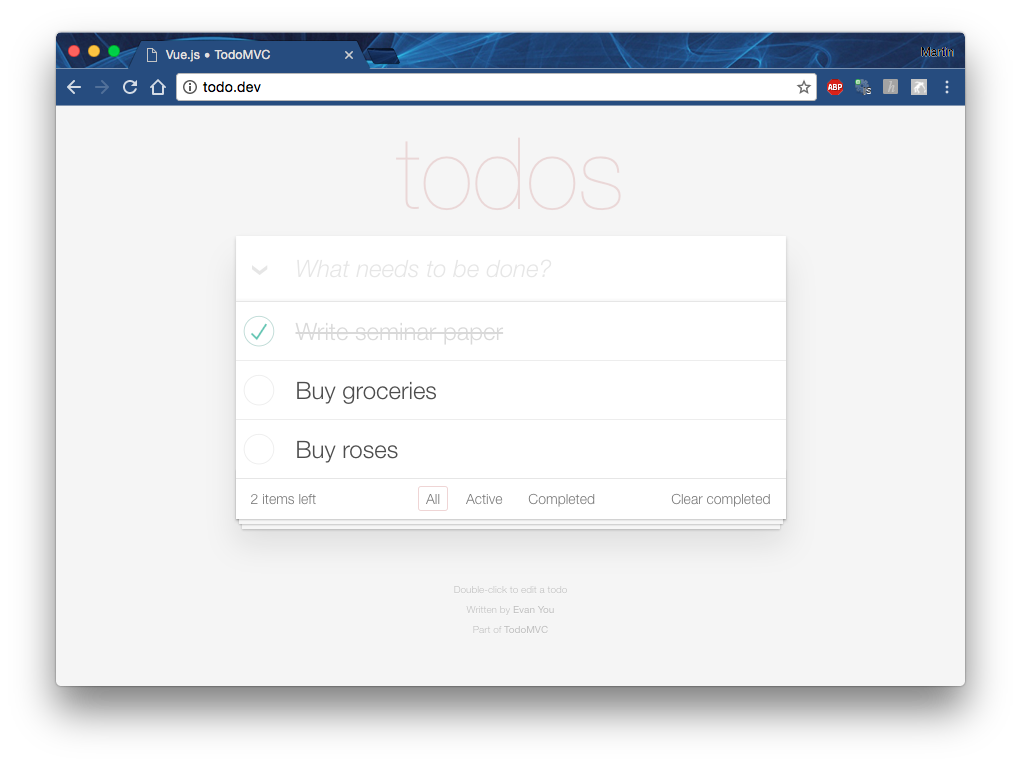
\includegraphics[width={\textwidth}]{img/vue-js-todo-filled.png}
  \caption{Todos Application}
  \label{image:todos-filled}
\end{figure}
\subsection{Selenium IDE}
Testovanie uživateľského rozhrania pomocou Selenium \acs{IDE} je v skutočnosti jednoduchý ale zdĺhavý proces. Najskôr je potrebné nainštalovať si doplnok Selenium \acs{IDE}\footnote{\url{https://addons.mozilla.org/sk/firefox/addon/selenium-ide/}} pre internetový prehliadač Firefox. Po úspešnom nainštalovaní doplnku treba doplnok zapnúť (alebo nechať zobraziť), a to tak, že v hornej lište prehliadača Firefox prejdeme na zložku Tools a následne vyberieme z menu Selenium \acs{IDE}, výsledkom čoho je zobrazenie ako na obrázku č. \ref{image:selenium-ide}.

Proces testovania spočíva v postupnom preklikávaní sa todos aplikáciou, pričom je zapnuté nahrávanie v prostredí Selenium \acs{IDE}. Výsledkom nahrávania akcií je HTML súbor (tabuľka), ktorý obsahuje jednotlivé akcie ako napríklad: \texttt{openWindow}, \texttt{verifyTitle}, \texttt{click}, \texttt{type}, \texttt{sendKeys} a iné\footnote{\url{http://seleniummaster.com/sitecontent/index.php/introduction-to-selenium-automation/selenium-ide/114-selenium-ide-complete-list-of-commands}}, spolu s parametrami, ktoré Selenium \acs{IDE} zachytilo pri vyklikávaní (alebo písaní textu, pohybu kurzoru myši a iné). 

Selenium \acs{IDE} vyhodnocuje úspešnosť daného testu (sekvenciu akcií) spôsobom, či sa vôbec daný test dá spustiť to znamená, že ak má Selenium \acs{IDE} v teste akciu ``klikni na tlačítko s id=add'', no reálne také tlačítko nie je nájditeľné v \acs{DOM}--e, celý test je označený ako ``neprejdený''. 

V tabuľke č. \ref{table:action-list-ide} je (skrátený) zoznam akcií, ktoré rozhodujú o úspešnosti testu. Samotný test uložený v súbore \texttt{application/selenium-ide-TODO}\footnote{\url{https://github.com/Kyslik/asos-selenium/blob/master/application/selenium-IDE-todo}}.

\begin{table}[h]
\centering
\caption{Zoznam akcií v teste pri použití Selenium IDE}
\label{table:action-list-ide}
\begin{tabular}{lll}
\textbf{akcia}   & \textbf{parameter}         & \textbf{parameter--2}    \\
otvor okno       & http://todo.dev 			  & --                       \\
verifikuj nadpis & Vue.js   TodoMVC           & --                       \\
napíš do         & input.new-todo             & Write presentation       \\
zmačkni          & ENTER                      & --                       \\
napíš do         & input.new-todo             & Watch Die Hard Movie \#3 \\
zmačkni          & ENTER                      & --                       \\
klikni na        & link=Active                & --                       \\
klikni na        & link=Completed             & --                       \\
klikni na        & css=button.clear-completed & --                       \\
zavri okno       & --						  & --                        
\end{tabular}
\end{table}
\subsection{Selenium 2}
Pre demonštráciu Selenium 2 (WebDriver) som sa rozhodol použiť jazyk PHP, ktorý nepotrebuje kompiláciu a má jednoduchú syntax.

Knižnica php-webdriver je obal (wrapper) pre Selenium WebDriver v jazyku PHP z dielne Facebook-u, ktorá umožnuje kontrolu respektíve ovládanie internetových prehliadačov priamo z PHP \cite{php-webdriver-facebook}. V dokumentácií\footnote{\url{https://github.com/facebook/php-webdriver/wiki}} php-webdriver-u je dôsledne popísaný postup ako s ním pracovať.

PHPUnit je najpopulárnejší\footnote{\url{http://www.hongkiat.com/blog/automated-php-test/}} framework na vykonávanie automatizovaných testov v jazyku PHP. Pre všetky testy vo frameworku PHPUnit platí, že pred každým testom sa spustí metóda \texttt{setUp()} a po ukončení testu metóda \texttt{tearDown()}, to znamená, že každý test je ``spustený vo vákuu'' (jednotkový test).
Konkrétnejšie v demonštračnom zdrojovom kóde v metóde \texttt{setUp()} sa nastaví: spojenie (so selenium-webdriver-serverom), prehliadač (typ) a jeho vlastnosti (napr. velkosť okna) a v metóde \texttt{tearDown()} je kód na zatvorenie okna internetového prehliadača.

Kompletný návod ako nainštalovať a rozbehať testovaciu aplikáciu spolu s PHPUnit a Selenium 2 je popísaný v prílohe \ref{prerequisites}.

V tabuľke č. \ref{table:test-list-selenium-2} je (úplný) zoznam testov, ktoré testujú todos aplikáciu.
\begin{table}[h]
\centering
\caption{Zoznam testov pri použití Selenium 2}
\label{table:test-list-selenium-2}
\begin{tabular}{ll}
\textbf{názov testu}     & \textbf{vysvetlenie}                           \\
TodoAppHome              & Testuj dostupnost aplikácie (http://todos.dev) \\
AddingTodos              & Testuj pridávanie úloh                         \\
MarkingAsComplete        & Testuj označenie ako úlohu ako ``splnenú''     \\
DestroyingTodo           & Testuj vymazanie úlohy                         \\
EditingTodo              & Testuj editovanie úlohy                        \\
MakeAnEditToTodo         & Testuj vykonanie zmeny úlohy (po editácii)     \\
SeeAllTodos              & Testuj filtrovanie úloh (filter ``všetky'')    \\
SeeActiveTodos           & Testuj filtrovanie úloh (filter ``aktívne'')   \\
SeeCompletedTodos        & Testuj filtrovanie úloh (filter ``splnené'')   \\
ClearCompletedTodos      & Testuj vymazanie ``splnených'' úloh            \\
CheckAllTodosAsCompleted & Testuj označenie všetkých úloh ako ``splnené'' \\
CheckAllTodosAsActive    & Testuj označenie všetkých úloh ako ``aktívne''             
\end{tabular}
\end{table}
\subsection{Porovnanie Selenium IDE a Selenium 2}
\noindent Prácu so Selenium IDE by som zhrnul do nasledovných bodov:
\begin{quote}
\begin{description}
\item[plus] jednoduché na používanie
\item[plus] nepotrebuje žiaden server (selenium-webdriver-server)
\item[mínus] funguje iba na internetovom prehliadači Firefox
\item[mínus] veľmi pomalé testovanie (vykonanie testu trvá dlho)
\end{description}
\end{quote}

\noindent Prácu so Selenium 2 by som zhrnul do nasledovných bodov:
\begin{quote}
\begin{description}
\item[plus] vhodné pre programátorov
\item[plus] podporuje veľké množstvo internetových prehliadačov
\item[plus] podporuje veľké množstvo programovacích jazykov (Java, Python, Ruby)\footnote{\url{http://docs.seleniumhq.org/docs/03_webdriver.jsp}}
\item[plus] oveľa rýchlejšie vykonenie testov (v porovnaní so Selenium IDE) 
\item[mínus] potreba študovať dokumentáciu
\end{description}
\end{quote}